\subsection*{Characteristics of Technologies} 
\phantomsection
\addcontentsline{toc}{subsection}{Characteristics of Technologies}
\label{subsection:characteristics}

In this study, we employ the HH algorithm to derive quantitative indicators that characterize each technology (see Methods\nameref{section:Methods}). 
First, we define ubiquity (or degree centrality) $K_{T,0}$ as the number of corporations connected to a technology; a lower value indicates that the technology is more exclusive. Similarly, the average diversity $K_{T,1}$, which measures the variety of corporations connected to a technology, implies that a higher value reflects diversified publication, whereas a lower value suggests specialization. In many cases, the average of each indicator is used as a threshold to distinguish high from low values \cite{Hidalgo2009,balland2017tci}.

Another key indicator is the TCI, which represents the sophistication required to produce a technology. A threshold of zero divides TCI into high and low categories: a high TCI implies that a technology demands a complex combination of unique inputs and advanced technical expertise which explains why only a few advanced corporations can publish it competitively, whereas a low TCI indicates reliance on widely available capabilities, allowing many corporations to participate.

To analyze the structure of corporate patent publication as depicted by the bipartite graph, we focus on the relationships among these three indicators. The mapping of technologies is based on the Schmoch system \cite{Schmoch2008} (Panel A in Fig.~\ref{fig:scatter}), where $K_{T,1}$ and $K_{T,0}$ are divided by their mean values, and TCI is segmented by a zero threshold.

% \paragraph{Relationship Between Ubiquity and Average Diversity.}
Panel B in Fig.~\ref{fig:scatter} shows that there is no correlation between $K_{T,0}$ and $K_{T,1}$ (Pearson correlation coefficient $r=0.064$), suggesting that technologies widely held by corporations do not necessarily correspond to more diversified production portfolios. 
In particular, the lower-left quadrant of Panel B represents sectors with both low ubiquity and low corporate diversification. For example, sectors corresponding to Electrical Engineering are predominantly located in this quadrant.

% \paragraph{Correlation Between Ubiquity and TCI.}
On the other hand, Panel C in Fig.~\ref{fig:scatter} reveals a moderate positive correlation between $K_{T,0}$ and TCI (Pearson correlation coefficient $r=0.594$). 
In this context, Electrical Engineering exhibits low ubiquity, low average diversity, and low TCI values, indicating that corporations in this field tend to concentrate their innovation efforts within narrowly defined domains.

% \paragraph{Detailed Analysis by IPC Classification.}
The relative positioning of technologies is further confirmed using a finer classification based on International Patent Classification (IPC) classes (SI Fig.~\ref{fig:persector}). 
Focusing on the five sectors defined by Schmoch \cite{Schmoch2008}, we observe that in four sectors the relationship between ubiquity and average diversity is either negligible or moderately correlated. Notably, the Electrical Engineering sector exhibits a clear positive correlation between ubiquity and TCI (Pearson correlation coefficient $r=0.738$), indicating that among corporations specializing in Electrical Engineering, some produce a comprehensive range of ubiquitous technologies while others focus on rare, specialized ones.

% \paragraph{Contrasting Chemical and Pharmaceutical Sectors.}
In contrast to Electrical engineering technologies, Chemistry and Pharmaceuticals technologies mostly exhibit high TCI and the high average diversity (Panel D in Fig.~\ref{fig:scatter}, Pearson correlation coeffecience $r=0.316$).
These sectors are characterized by rarity and high sophistication and are typically developed by more diversified corporations. 
Moreover, corporations in these domains are connected not only to fields with low ubiquity but also to those that are more common (e.g., Biotechnology, Analysis of Biological Materials, and Measurement as shown in the right quadrant of Panel C in Fig.~\ref{fig:scatter}). 
A detailed examination reveals a slight negative correlation between ubiquity and average diversity (SI Fig.~\ref{fig:persector}), suggesting that in sectors with high technological complexity, corporations with more comprehensive technological portfolios tend to produce rare technologies. 
Furthermore, the IPC classes corresponding to Biotechnology and Measurement, show high TCI values in fields related to the production of sugar and yeast (C13, A21, C12), drug discovery (A61), and the preservation and management of these technologies (C07, A23). These findings are consistent with the socio-technical context of the period, particularly reflecting the emergence of drug discovery technologies in the 1980s and 1990s \cite{Sakakibara2014,Nakamura2022}. Moreover, the significant roles of food chemistry and biotechnology during the 1990s and 2000s underscore their contribution to the development of additives that enabled safer food preservation and processing not only in Japan but globally \cite{Bhatia2018,Murakami2024}.

\begin{figure}[ht]
    \centering
    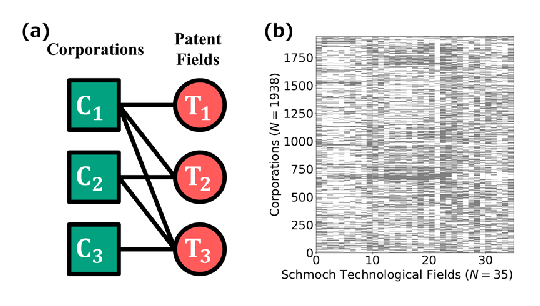
\includegraphics[scale=1.00]{Figs/Fig1.eps}
    \caption{(A) The legend of the five classifications defined by Schmoch \cite{Schmoch2008}, along with an explanation of the technology codes used in (B), (C), and (D).
    (B) Pearson correlation between \(K_{T,0}\) and \(K_{T,1}\) (\(r=0.064\)).
    (C) Pearson correlation between \(K_{T,0}\) and TCI (\(r=0.594\)).
    (D) Pearson correlation between TCI and \(K_{T,1}\) (\(r=0.316\)).
    The black lines indicate the mean values of \(K_{T,0}\) and \(K_{T,1}\), and \(\text{TCI} = 0\) is also shown with a black line. Each dot is color‐coded according to (A).
    }
    \label{fig:scatter}
\end{figure}
